\cxset{
 name={CHAPTER},
 numbering=arabic,
 number font-size=\Large,
 number font-family=\rmfamily,
 number font-weight=\normalfont,
 number before=,
 number after=\hspace{1em}\hfill\hfill\par\vspace*{20pt}\centerline{\textcolor{purple}{\decoone}}\vspace*{20pt},
 number dot=,
 number position=rightname,
 name=CHAPTER,
 chapter font-family=\rmfamily,
 chapter font-weight=\normalfont,
 chapter font-size=\Large,
 chapter before={\vspace*{20pt}\par\hfill},
 chapter after={},
 chapter color= black!90,
 number color= black!90,
 title beforeskip={},
 title afterskip={\vspace*{50pt}\par},
 title before={\hfill},
 title after={\hfill\hfill},
 title font-family=\rmfamily,
 title font-color= black!90,
 title font-weight=\normalfont,
 title font-size=\Huge}

\chapter{Introduction to Chapter Style Eighteen}

\parindent0pt
This design introduces an ornament. There are a number of packages on ctan that provide ornaments. If you using XeLaTeX it is also possible to use system fonts. The ornament is introduced with the key number after. At this point also we introduced all the vertical skips.
\medskip
\begin{figure}[ht]
\centering
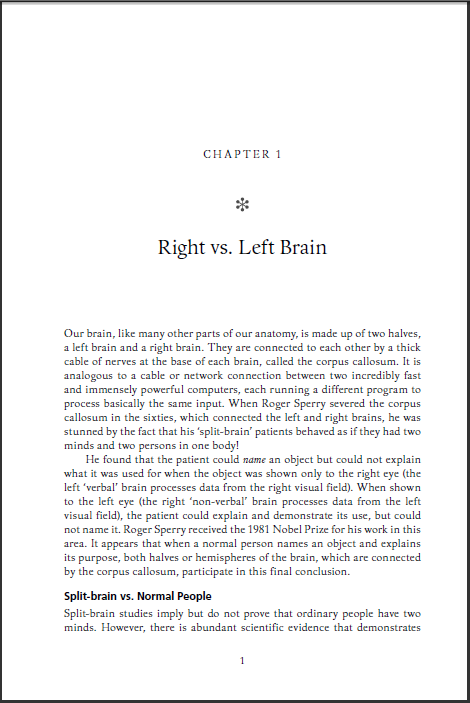
\includegraphics[width=0.45\textwidth]{./chapters/chapter18}
\end{figure}
